%!TEX root = ../master.tex
\section{Functional programaing}

\subsection{(Untyped) Lambda Calculus}
\label{Lambda Calculus}
$\lambda$-calculus is a formal system for expressing computation made by Alonzo Church. It consists of terms, and binding and substitution over terms. To build terms there are three rules:

\begin{itemize}
    \item Variable: A name which  is a placeholder for a parameter. An variable $x$ is in itself a lambda term 
    \item Abstraction: If we have a term $M$ and an variable $x$. Then we also have the term $\lambda x.M$ where $x$ is bound in the expression
    \item Application: If $E_1$ and $E_2$ are lambda-terms then $(E_1 E_2) $ are also a lambda term. Where $E_2$ is applied to $E_1$
\end{itemize}
All functions in $\lambda$-calculus are first-class values, which means that you can send in a function as an parameter, and that a function can return a other function (or the same function, ref. to the self-application function ($\lambda f.ff$)). It can also be good to know that $\lambda$-calculus is left-associative this means that $E_1 E_2 E_3 \leftrightarrow E_1 (E_2 E_3)$  \\ \\
To make it easier to understand the the different theologies used and explained in the sections bellow look at the figure \nameref{fig:LC-explenations}. 

\begin{figure}
    \centering
    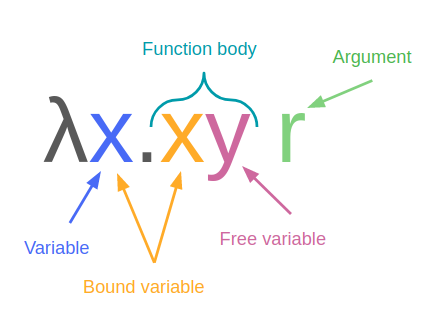
\includegraphics[scale=0.4]{lambdaCalculusFunctionExplenation.png}
    \caption{Explanations of the different 
theologies in $\lambda$-calculus}
    \label{fig:LC-explenations}
\end{figure}


\subsubsection{Lambda terms}
The rules to make terms is all ready explained in the previous chapter. But I want to add some extra information. Among other things that the \textbf{abstraction} rule is the rule that makes the definition of the anonymous function. Furthermore the abstraction in it self only makes the function and binds the variables, but it doesn't execute it. 

\subsubsection{Bound and Free variables}
As previously mentioned it is the \textbf{abstraction} that sets the \textbf{bound variables}, namely the $\lambda$ in the term binds the variable, and an variable is bound if it is found in the body of the abstraction. E.g the variable $x$ is a \textbf{bound variable} in the abstraction of the $\lambda$-term $\lambda x.x$.\\ \\
The \textbf{free variables} are the opposite the bound variables, or said with other words the rest of the variables. Said more formal: If you have a set of bound variables $B_1$ in a term $E_1$ with a set $V_1$ for all variables.  Then the free variables $F_1$ are $F_1 = \{V_1\setminus B_1\}$. 
You can also extend this general rule further, let us add another therm $E_1$ with a set $V_2$ for all variables in the term and $B_2 $ for all the bound variables. Then the \textbf{free variables} in $E_1 E_2$, $F_1 F_2$ is $F_1 F_2 = \{V_1\setminus B_1\} \cup \{V_2\setminus B_2\}$. In other words the set of the free variables in term $E_1 E_2$ is the union of the free variables in $E_1$ and $E_2$
To further elaborate you can state that if you have a term which consist of the free variable $x$, then $x$ is a free variable.

\subsubsection{$\alpha$-conversion}

First of it is nice to mention what \textbf{$\alpha$ equivalence} is. It basically means that that two lambda terms are alpha-equivalent if the one 
difference in the terms has the variables names. E.g $\lambda ab.ab$ is alpha-equivalent to the lambda term $\lambda xy.xy$ 
\\ \\
With the $\alpha$-reduction in mind, \textbf{$\alpha$-conversion} is that you change the name of the variable in the $\lambda$ part 
and in the body so that the new term is $alpha$ equivalent to the old term. E.g on $\alpha$-conversion of $\lambda ab.ab$ is $\lambda xy.xy$ 
since this are $alpha$ equivalent. Bear in mind that you're not allowed to rename the variable to a name of another variable in the term. 
This because the two terms won't be $alpha$ equivalent.

\paragraph{$\alpha$-conversion exampels}. As we have allready mention when doing $\alpha$-conversion we can only change the names of the variables in the term, so that 
the term dosen't change. E.g. $\lambda x.x \rightarrow_\alpha \lambda y.y$ since we haven't change the meaning of the term. So the reuslt of sending in any value/term 
$e$ will give ous the same reutrn value, in this case just $e$ itself. An exampel of what isn't allowed to do is this $\lambda x.xy \rightarrow_\alpha \lambda y.yy$. This is 
because this terms will give us different return values for an arguemnt. Lets try with $e$ again, then we would se that  $\lambda x.xy e$ would give us $ey$ while 
$\lambda y.yy e$ whould give us $ee$, and $ey \neq ee$. So the term $\lambda x.xy$ is $\alpha$-equivalent to all terms where we change to $x$ to any thing except $y$. 
More general we can change any variable name to anything except the set of variables in the function body. Therefore $\lambda x.xy \rightarrow_\alpha \lambda z.zy$.
In addition we need make sure that vi only change the variables that are in the same abstraction. So the term $\lambda x.\lambda x.x $ is not $\alpha$-equivalent to the 
term $\lambda y.\lambda x.y$, but to for exampel the terms $\lambda y.\lambda x.x$ or $\lambda x.\lambda y.y$

\subsubsection{$\beta$-reduction}
$\beta$-reduction is a way to reduce terms. You do this by sending in argument(s) for the bound variables. E.g. if we want the reduce the lambda term $\lambda x. x s$ we can $\lambda x. x$  $s \rightarrow _\beta s$ (this is the identity function, which gives us back the argument we gave to the function). You can do $\beta$-reduction in several rounds, when there are no more possible $\beta$-reductions we say that the term has reached the $\beta$-normal form. Figure 2: \nameref{fig:beta-reduction} shows an example on $\beta$-reduction with a $\lambda$-term of one of the arguments. \\ \\
If the term stays the same after one $\beta$-reduction, then the term never will terminate. An example of a term that doesn't terminate wail using $\beta$-reduction is the self-application function applyed on itself $(\lambda f.ff) \lambda f.ff$

\paragraph{Complexity}
$\beta$-reduction is not an atomic step, this means that one most locate all the occurrence of a bound variable in a term, which can be very time consuming. In O-notation this will take $O(n)$ time for a term of length n. On way to this is to store this value some place, this may become very space costly. 

\begin{figure}
    \centering
    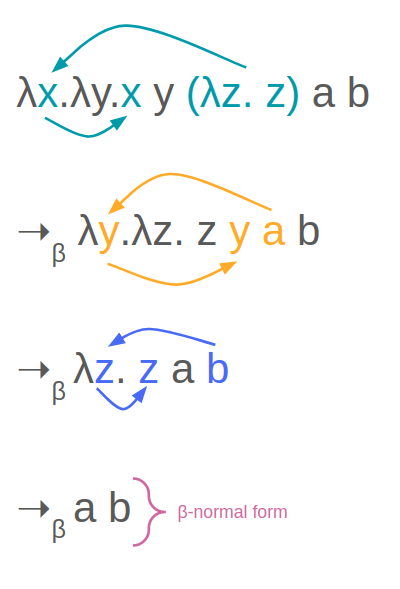
\includegraphics[scale=0.4]{b-reduction.png}
    \caption{An example of $\beta$-reduction}
    \label{fig:beta-reduction}
\end{figure}

\subsubsection{$\eta$-reduction}
$\eta$-reduction is the idea that two functions are equal if and only if they returns the same result for 
any given argument. An example of $\eta$-reduction is $(\lambda x.f x)  \rightarrow_\eta f$, whenever $x$ is not 
a free variable in $f$.

\subsection{Type Theory}
\label{Type Theory}
Type theory is the academic study of \textbf{type systems}, 
which gives every term a type. This type chooses what operations 
that can be done on the term, as well as the meaning of it. 
\nameref{Lambda Calculus} has it's own type system, also made 
by Alonzo Church called \nameref{Simply Typed Lambda Calculus}.
\\ \\
\textbf{A term} often followed by a : and then the type of the term.
\textbf{A type} in a type system is semantically often collection of different
values that a term can be evaluated to. Therefore, there are many 
similarities between type systems and set theory, eventhrough they 
have their differences. Futher more the name of a given term is the syntactic, 
for exampel in java we have the type that  is a collection of all Integers ($\mathbb{Z}$) (semantic) 
and has the name int (syntactic).
So a term $e$ ($e$ is often use to denote a term) is of type 
$\tau$ ($\tau$ is often use to denote a type) if $e \in \tau$. 
E.g. 2 is of type $\mathbb{N}$ (natural numbers) because 
$2 \in \mathbb{N}$. Often terms and types are made depending on their 
type system which we will come back to when we talk about \nameref{Simply Typed Lambda Calculus}
$\Upgamma \vdash e:\tau$ is the denotation of a judgment. 
Where $\Upgamma$ is the denotation that usually is used for an 
context or environment. A terms typed is determinate using the 
judgment and equivalences type inference rules. 
\\ \\
Many of the programming languages either requiere that all expressions terminate (e.g. Coq) or alow 
infinitete loops but are inconsistent when viewed as logics (e.g. Haskel) \textbf{(src: http://www.tyconmismatch.com/papers/combining-TR.pdf)}.
Therefore in some programaing languages, like \nameref{Simply Typed Lambda Calculus}, one of the type systems goals 
is to make sure that a term terminates. 
\\ \\
Many type systems have \textbf{inductive types}. Among other things this means that we have a set of base types
and a set of type constructors that again can generate new types. So if we have the base typee $\sigma$ , 
and two opertions $*$ and $\#$ and with the types $M$ and $N$ (what they mean are not important for this exampel) 
then we can make a new type $T$ in the ways in \nameref{tab:inductive types} 

\begin{table}[]
    \centering
    \begin{tabular}{c c c}
         $T :=$&  & $\sigma$\\
         & $|$ & $M * N$ \\
         & $|$ & $M \# N$ \\
    \end{tabular}
    \caption{Example of how to build up inductive types}
    \label{tab:inductive types}
\end{table}


\subsubsection{Decision problems}

Type theory uses type checking, typebility and type inhabitation as decisions problems. \\ \\
The decision problem of \textbf{checking} (abbreviated by ($\Upgamma\vdash e : \tau$?) is:\\
\textit{Given a type environment $\Upgamma$, a term $e$, and a type $\tau$, decide whether the term $e$ can be assigned the type $\tau$ in the type environment $\Upgamma$} \\ \\
The decision problem of type \textbf{typability} (abbreviated by ($ \exists \Upgamma,\tau .\Upgamma\vdash e : \tau$?) is: \\ 
\textit{Given  a term $e$, decide wheter there exists a type environment $\Upgamma$ and a type $\tau$ such that the term $e$ can be assigned the type $\tau$ in the type environment $\Upgamma$} \\ \\ 
The decision problem of type \textbf{inhabitation} (abbreviated by ($ \exists e.\Upgamma \vdash e : \tau$?) is: \\
\textit{Given a type environment $\Upgamma$ and a type $\tau$, decide whether there exists a term $e$ that can be assigned the type $\tau$ in the type environment $\Upgamma$}

\subsection{Simply Typed Lambda Calculus}
\label{Simply Typed Lambda Calculus}
As earlier mention in the section about \nameref{Type Theory}, Simply Typed Lambda Calculus 
($\lambda^\rightarrow$) is an Type Theory developed by Alonzo Church for $\lambda$-calculus. \\ \\
In $\lambda^\rightarrow$ we can make types with only on operator $\rightarrow$ and a set of base types,
 often denoted with $B$. From the base types, $B$, we can construct new types using our operator 
 $\rightarrow$. If we have the two base types $\tau$ and $\sigma$ we can construct a new 
 type $\tau \rightarrow \sigma$, this type that we now just made would refer to a function 
 that takes in an argument of type $\tau$ and returns a term of type $\sigma$. \\ \\
The syntax for $\lambda^\rightarrow$ are more or less equal to \nameref{Lambda Calculus}s syntax. 
Except that we need to specify the type of an variable in the function (in the abstraction), 
this is done in the way that was described in \nameref{Type Theory} with $x:\tau$ for an variable $x$ with 
type $\tau$. In addition Simply type lambda calculus also adds a term constant $c$. The full syntax for 
Simply Typed Lambda Calculus is shown in the table \nameref{tab:STLC syntax} \\

\begin{table}[]
    \centering
    \begin{tabular}{c c c}
         $e :=$&  & $x$\\
         & $|$ & $\lambda x:\tau.M$ \\
         & $|$ &  $M N$ \\
         & $|$ &  $c$ \\
    \end{tabular}
    \caption{Simply Typed Lambda Calculus syntax}
    \label{tab:STLC syntax}
\end{table}

\subsubsection{Typing rules}
In Simply Typed Lambda Calculus we have four typing rules. To state this rules we need to take with us the typing environment 
that was described in the section about \nameref{Type Theory}.

\begin{enumerate}
    \item If we have variable $x$ that is of type $\tau$ in the typing environment $\Upgamma$, then we know that $x$ has type $\tau$.
    \item If we have a constant $c$ of type $T$ in the typing environment $\Upgamma$, then we know that $c$ has type $T$.
    \item If we have a variable $x$ that is of type $\tau$ in a type environment, and with a term $e$ of type $\sigma$ in the same type environment, then we have a term $\lambda x\tau .e$ with the type $\tau \rightarrow \sigma$ in the same type environment.
    \item If we have a term $M$ of type $\tau \rightarrow \sigma$ and a term $N$ of type $\tau$ in an typing environment, then $M N$ will have the type $\tau$ in the same typing environment.
\end{enumerate}

\subsubsection{Reduction of Simply Typed Lambda Calculus}
Simply Typed Lambda Calculus also uses the $\beta$-reduction and $\eta$-reduction as mention in the 
section in about \nameref{Lambda Calculus}, but we need to check that the arguments to the function has 
the right type in typing environment as well. 
\\ \\
To give an example of this we first need to make a set of the base types, in this case we wil only use $Int$, which is the name for the collection of all 
naturla numbers, as the only base type. From this one type we can make an infinity of types ($Int, Int \rightarrow Int, Int \rightarrow Int \rightarrow Int ....$).
In addtion we will add the operation $+$ that adds to numbers together.
We will use the term $e_1:= \lambda x:Int\: y:Int. + x y:Int \rightarrow Int \rightarrow Int$, the type $Int \rightarrow Int \rightarrow Int$ in writing would be "a term
which takes in an Int and returns a term which takes in an Int and returns an Int". 
So if we know apply the term $e_2 := 3:Int$ on $e_1$, $e_1 e_2$ from the third type rule we se that this the term 
$e_1 e_2$ should have the type $Int \rightarrow Int$. To show this let us use $\beta$-reduction on the terms.
\\ \\
$e_1 e_2 := \lambda x:Int\: y:Int. + x y:Int \rightarrow Int \rightarrow Int\; 3:Int 
\newline\rightarrow_\beta \lambda y:Int. + 3\; y: Int \rightarrow Int$
\\ \\
So the term we that $e_1 e_2 $ now is a term which takes in a $Int$ and returns an $Int$. If we apply another term
$e_3 := 7:Int$ on the term $e_1 e_2:Int \rightarrow Int$ we get the term $e_1 e_2 e_3:Int$ from the third typing rule.
The $\beta$ reduction also shows this: 
\\ \\
$e_1 e_2 e_3 := \lambda y:Int. + 3\; y: Int \rightarrow Int \; 7:Int
\newline \rightarrow_\beta + 3:int \; 7:Int = 10$

\subsection{Evaluation strategies}
An evaluation strategie is an stratagie that is used in programming languages to decide when
an expression should be evaluated. E.g should we evaluate the the arguments before the function, and send in 
the evaluated values as argumments as values, or should we should we just send the whole expression as an argumment 
and evaluate it later. Furthermore it has two main branches \textbf{eger evaluation} (strict evaluation) and \textbf{non-strict evaluation}, to explain briefly 
eger evaluation will evaluate the expression at soon as it is bound, considering the example given earlier eger evaluation whould evaluate every 
argument before it starts the function. Non-strict evaluation on the other hand evaluates the expression when it's
first used. This means that if you have a function that takes an argument that is never used eger evaluation will evaluate it while 
non-strict evaluation wouldn't. Non-strict evaluation can also have infinit list, since only the element in the list which are used are 
calculated, infinit list is also known as streams. 
\\ \\
Most Imperative programming languages uses an eger evalutation. In imperative languages the order of how the code is 
executeted is determined by the structur ande the order of code itself. The reason we eager evaluation is the most popular 
evaluation strategie in imperative programming languages is because it easier to avoid unexepted behavoir.  In addition to being eaiser to 
debug compared with non-strict evalutation. One can also have some diffuclites when it trying to use imperative features like I/O and exception handling 
when using a non-strict evaluation strategie. Even though most imperative languages is writen using eger evalutation it still have some non-strict evaluation element in it. 
A good exampel of this is the if-statment where the most languages only will evaluate the one part of the if-statment that is true. If we have $if\; a\; then\; b\; else\; c$, then b only 
will evaluated if a is evaluates to be true, and c on the other hand wil only be evaluated if a is evaluated to be false. But if we put this if-statment in a function and use $a$, $b$ and
$c$ as arguments like this $f(a, b ,c):= \; if\; a\; then\; b\; else\; c$ then eger evaluation will evaluate all the expressions before the functions starts even though we 
know we only need either $b$ or $c$ while non-strict evaluation only whould evaluate the expression that is used.
\\ \\
\textbf{Lazy evaluation} (also know as call-by-need) is a subbranch 
of non-strict evaluation and often used in Functional programming. Since Lazy evaluation is a subbranch of non-strict it evaluates 
the expression when it is used. What seperating lazy evaluation from the other types of non-strict evaluation such as call-by-name
is that Lazy evalutation also use memorization to avoid repeated evaluations, ruducing the running time. Memorization is done by using a 
look-up table where you store the value of what a function for a some given arguments evaluates to. When you then whant to evaluate a 
function with som arguments you first check if it allready exists in the look-up table, if the value exists you can retrive it form the table, on the 
other hand if doesn't exist you evaluate the function to a value and add this value to the table.
\textbf{Graph reductuion} is an efficant technique for implementing lazy evaluation using the outermost tree reduction method.
\\ \\
In figure \nameref{fig:strictVSLazy} we se an exampel of strict evaluation and lazy evaluation with $\beta$-reduction, with the 
assumtion that print is a term which prints the argument to the terminal, and that + - and * are operators that works on integers.
There are some differences that are important to note:

\begin{itemize}
    \item In strict evaluateion we evaluate a as soon as its bond, will we don't do it in lazy evaluation.
    \item In strict evaluation we evaluate the terms before sending them in while we in lazy evaluation send in the whole term
    ref. $(\lambda x.\lambda y. - x y)\; 4 \; 2$. Since we never uses the $y$ anywhere in the function body the result is that 
    in strict evaluation ends up evaluating something that never is used.
    \item On the last to lines on the Lazy Evaluation we can se that we have used memorization and the lookup table to get
    the return value, instead of calculating it twice.
\end{itemize}

\begin{figure}
    \centering
    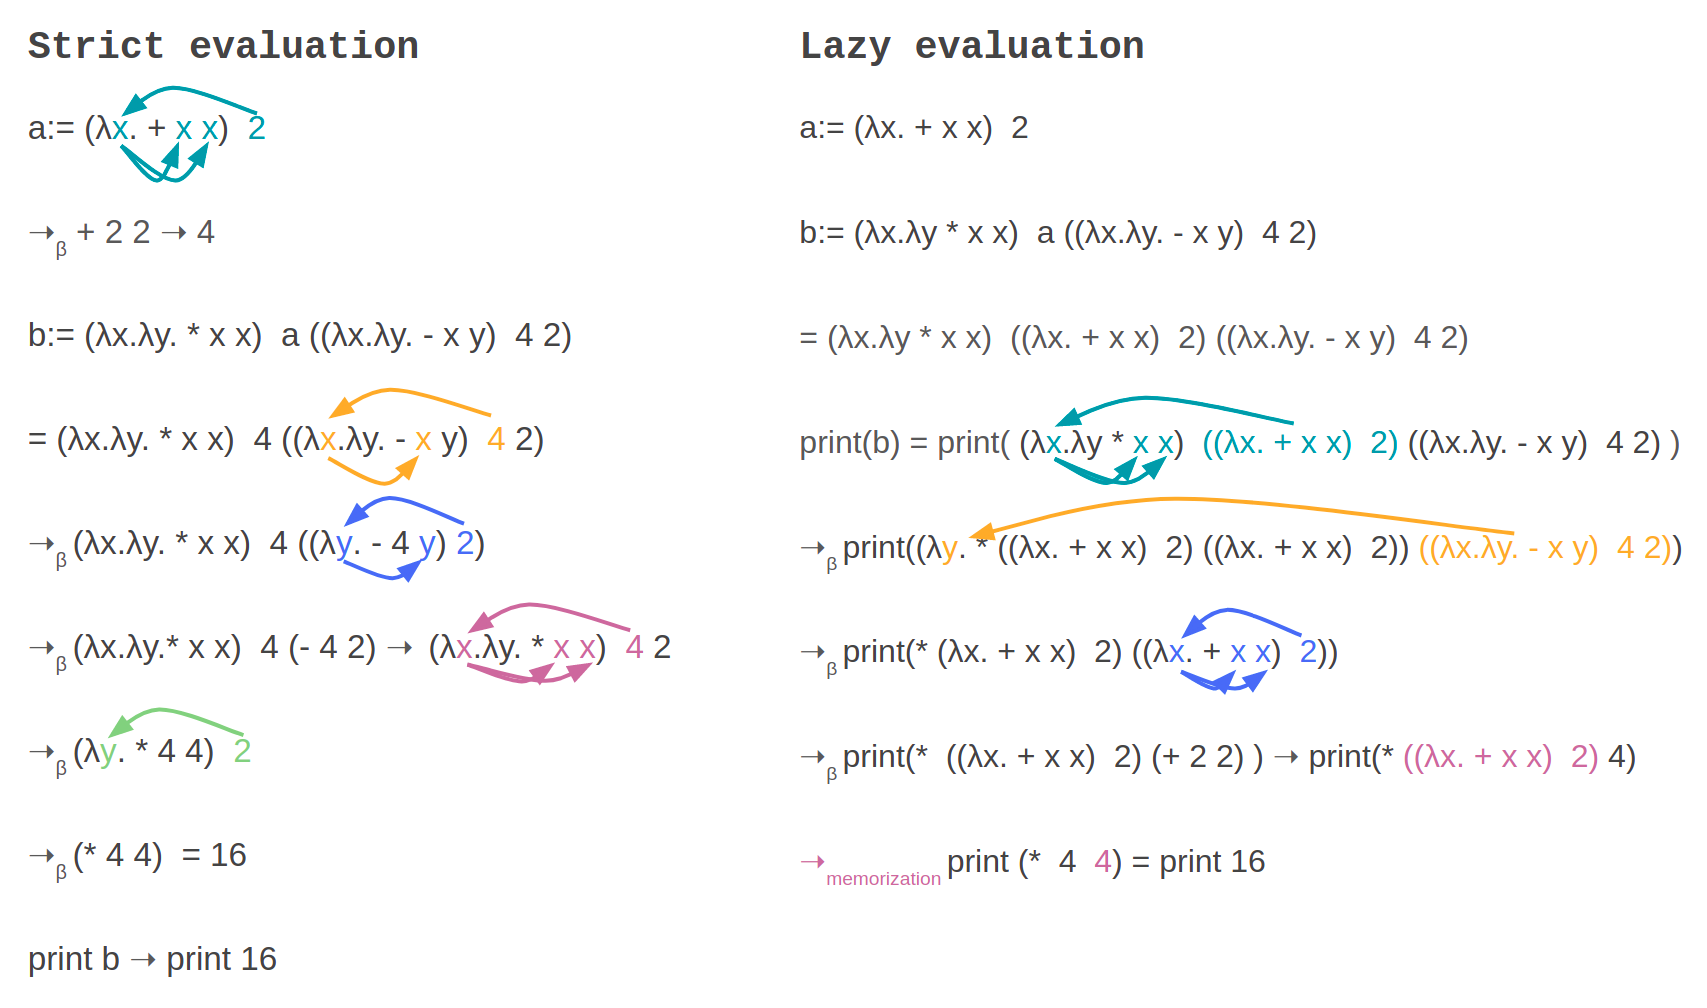
\includegraphics[scale=0.25]{strictVSLazy.png}
    \caption{Shows the diffetence between strict evaluation and lazy evaluation. Here we assum that print is a term which 
    prints the argument to the terminal, and that + - and * are operators that works on integers}
    \label{fig:strictVSLazy}
\end{figure}